\documentclass[11pt]{article}

\usepackage[margin=1in]{geometry}
\usepackage{amsmath, amssymb, amsthm}
\usepackage{microtype}
\usepackage{xcolor}
\usepackage{hyperref}
\usepackage{enumitem}
\usepackage{parskip}
\usepackage{tikz}
\usetikzlibrary{arrows.meta, positioning}

\hypersetup{
  colorlinks=true,
  linkcolor=blue!60!black,
  urlcolor=blue!60!black,
  citecolor=blue!60!black
}

\newcommand{\R}{\mathbb{R}}
\newcommand{\N}{\mathbb{N}}
\newcommand{\sci}{\chi'_s}

\newtheorem*{conjecture*}{Conjecture}
\newtheorem*{theorem*}{Theorem}
\newtheorem*{prop*}{Proposition}

\title{\textbf{The Strong Chromatic Index and the Erd\H{o}s--Ne\v{s}et\v{r}il Conjecture}}
\author{}
\date{}

\begin{document}
\maketitle

\vspace{-2em}

\section*{The setup, with pictures (start here if you need it)}

\subsection*{Graphs: dots and lines.}

A \emph{graph} $G$ is a finite set of \emph{vertices} (dots) together
with a set of \emph{edges} (lines) joining some pairs of vertices.
That is it. No coordinates, no geometry --- just ``which dots are
joined by a line.'' Here is a graph with $5$ vertices and $6$ edges:

\begin{center}
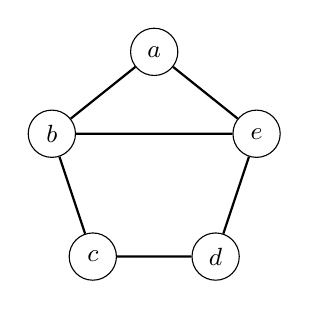
\begin{tikzpicture}[scale=1.3, vtx/.style={circle, draw, fill=white, inner sep=1.5pt, minimum size=6mm, font=\small}]
  \node[vtx] (a) at (0, 1.2)    {$a$};
  \node[vtx] (b) at (-1, 0.4)   {$b$};
  \node[vtx] (c) at (-0.6, -0.8){$c$};
  \node[vtx] (d) at (0.6, -0.8) {$d$};
  \node[vtx] (e) at (1, 0.4)    {$e$};

  \draw[thick] (a) -- (b);
  \draw[thick] (a) -- (e);
  \draw[thick] (b) -- (c);
  \draw[thick] (c) -- (d);
  \draw[thick] (d) -- (e);
  \draw[thick] (b) -- (e);
\end{tikzpicture}
\end{center}

\subsection*{Degree, and what $\Delta(G)$ means.}

The \emph{degree} of a vertex $v$, written $\deg(v)$, is the number of
edges that touch it. Just count the lines coming out of the dot. For
the graph above:

\begin{center}
\begin{tabular}{c|cccccc}
vertex & $a$ & $b$ & $c$ & $d$ & $e$ \\
\hline
$\deg$ & $2$ & $3$ & $2$ & $2$ & $3$ \\
\end{tabular}
\end{center}

The \textbf{maximum degree} of $G$, written $\Delta(G)$, is the
largest degree of any vertex in $G$. For our example,
$\Delta(G) = 3$ (achieved by $b$ and $e$). That is the single most
important number describing a graph for our purposes.

\textbf{In words:} ``$\Delta(G) = k$'' means \emph{every vertex has
at most $k$ edges sticking out of it, and at least one vertex has
exactly $k$}.

\subsection*{Edge colouring: the easy version.}

A \emph{proper edge colouring} is an assignment of a colour to every
edge such that \textbf{any two edges meeting at the same vertex get
different colours}. That is the only rule.

\begin{center}
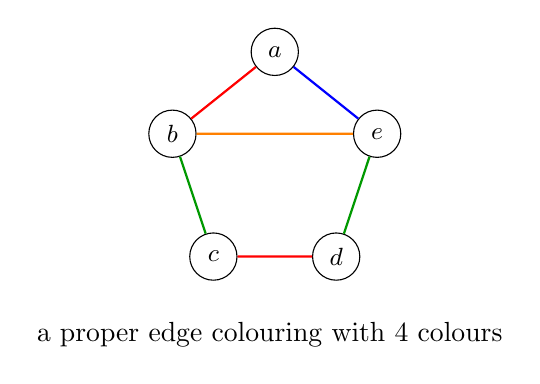
\begin{tikzpicture}[scale=1.3, vtx/.style={circle, draw, fill=white, inner sep=1.5pt, minimum size=6mm, font=\small}]
  \node[vtx] (a) at (0, 1.2)    {$a$};
  \node[vtx] (b) at (-1, 0.4)   {$b$};
  \node[vtx] (c) at (-0.6, -0.8){$c$};
  \node[vtx] (d) at (0.6, -0.8) {$d$};
  \node[vtx] (e) at (1, 0.4)    {$e$};

  \draw[thick, red]   (a) -- (b);
  \draw[thick, blue]  (a) -- (e);
  \draw[thick, green!60!black] (b) -- (c);
  \draw[thick, red]   (c) -- (d);
  \draw[thick, green!60!black] (d) -- (e);
  \draw[thick, orange](b) -- (e);

  \node[below=-2pt] at (-0.05, -1.4) {a proper edge colouring with 4 colours};
\end{tikzpicture}
\end{center}

The minimum number of colours that suffices is the
\emph{chromatic index} $\chi'(G)$. Vizing's theorem (1964) says
$\chi'(G)$ is either $\Delta(G)$ or $\Delta(G) + 1$. Cleanly bounded
by $\Delta(G)$.

\subsection*{Strong edge colouring: the hard version.}

A \emph{strong edge colouring} adds a second rule. Now:
\begin{itemize}[leftmargin=*, itemsep=2pt]
  \item Edges meeting at a vertex must get different colours (as before), \emph{and}
  \item Edges that are \textbf{joined by another edge} must \emph{also} get different colours.
\end{itemize}
Equivalently: every colour class must be an \emph{induced matching}
--- a set of edges with no two of them within ``one hop'' of each
other.

\begin{center}
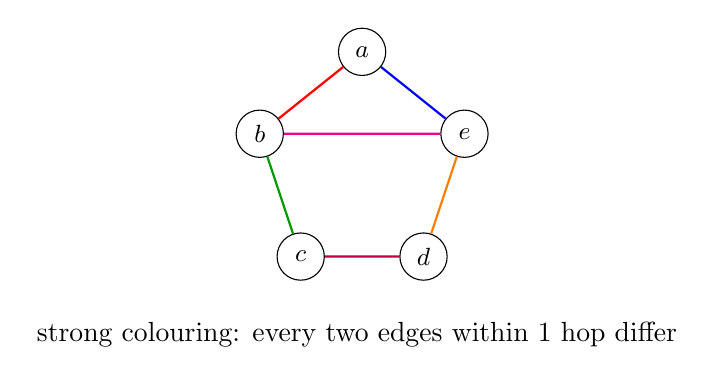
\begin{tikzpicture}[scale=1.3, vtx/.style={circle, draw, fill=white, inner sep=1.5pt, minimum size=6mm, font=\small}]
  \node[vtx] (a) at (0, 1.2)    {$a$};
  \node[vtx] (b) at (-1, 0.4)   {$b$};
  \node[vtx] (c) at (-0.6, -0.8){$c$};
  \node[vtx] (d) at (0.6, -0.8) {$d$};
  \node[vtx] (e) at (1, 0.4)    {$e$};

  \draw[thick, red]      (a) -- (b);
  \draw[thick, blue]     (a) -- (e);
  \draw[thick, green!60!black] (b) -- (c);
  \draw[thick, purple]   (c) -- (d);
  \draw[thick, orange]   (d) -- (e);
  \draw[thick, magenta]  (b) -- (e);

  \node[below=-2pt] at (-0.05, -1.4) {strong colouring: every two edges within 1 hop differ};
\end{tikzpicture}
\end{center}

For the graph above, the strong rule forces $6$ different colours
(every pair of edges is within one hop of each other, because the
graph is small). So $\sci(G) = 6$ here.

The minimum number of colours that makes a strong colouring possible
is the \emph{strong chromatic index} $\sci(G)$. This is the
quantity the rest of the paper is about.

\subsection*{One more picture: why $\sci$ blows up.}

Even though ordinary $\chi'(G)$ is at most $\Delta(G) + 1$, the
strong version $\sci(G)$ can be \emph{quadratic} in $\Delta(G)$ ---
much bigger. The reason is the
\emph{blow-up of $C_5$}, which we will keep returning to.

\textbf{$C_5[2]$:} take the $5$-cycle, replace each vertex with $2$
twin vertices, and join twins across the cycle. The result has
$10$ vertices, $20$ edges, every vertex has degree $\Delta = 4$,
and \emph{every pair of edges is within $1$ hop of each other}. So
every edge needs its own colour:

\begin{center}
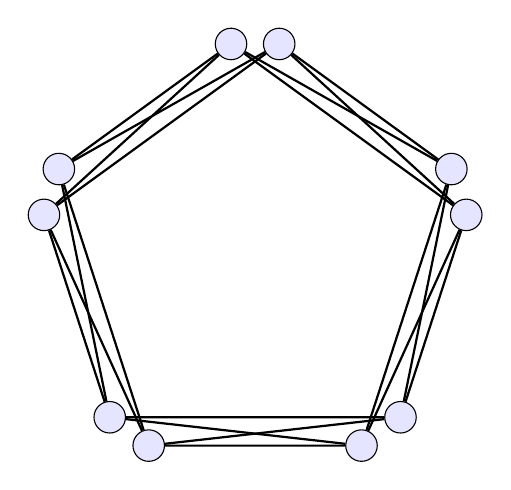
\begin{tikzpicture}[scale=1.7, vtx/.style={circle, fill=blue!10, draw, inner sep=1pt, minimum size=4mm, font=\scriptsize}]
  \foreach \i/\angle in {1/90, 2/162, 3/234, 4/306, 5/18} {
    \pgfmathsetmacro{\rx}{1.6*cos(\angle)}
    \pgfmathsetmacro{\ry}{1.6*sin(\angle)}
    \pgfmathsetmacro{\dx}{0.18*cos(\angle+90)}
    \pgfmathsetmacro{\dy}{0.18*sin(\angle+90)}
    \node[vtx] (V\i a) at (\rx+\dx, \ry+\dy) {};
    \node[vtx] (V\i b) at (\rx-\dx, \ry-\dy) {};
  }
  \foreach \i/\j in {1/2, 2/3, 3/4, 4/5, 5/1} {
    \draw[thick] (V\i a) -- (V\j a);
    \draw[thick] (V\i a) -- (V\j b);
    \draw[thick] (V\i b) -- (V\j a);
    \draw[thick] (V\i b) -- (V\j b);
  }
\end{tikzpicture}
\end{center}

So $\sci(C_5[2]) = 20 = 5 \cdot 4^2 / 4$. This is the conjectured
worst case for $\Delta = 4$. The Erd\H{o}s--Ne\v{s}et\v{r}il
conjecture says: \emph{no graph with $\Delta = k$ ever needs more
than $5k^2/4$ colours for a strong edge colouring}.

That is the conjecture. Everything after this section is about
trying to prove it.

\section*{Detour: a proof of Vizing's theorem}

Before diving into the \emph{strong} version, here is a self-contained
proof of the ordinary version. It is short, beautiful, and worth
seeing once.

\begin{theorem*}[Vizing, 1964]
For any simple graph $G$,
\[
\chi'(G) \;\leq\; \Delta(G) + 1.
\]
\end{theorem*}

The lower bound $\chi'(G) \geq \Delta(G)$ is trivial: the $\Delta(G)$
edges meeting a max-degree vertex must all receive different colours.
The interesting part is the upper bound.

\begin{proof}
Set $k = \Delta(G) + 1$. We show $G$ admits a proper edge colouring
with $k$ colours, by induction on $|E(G)|$. The base case
$|E(G)| = 0$ is trivial.

Let $e = xy_1$ be any edge of $G$. By induction, $G - e$ has a proper
edge colouring $c$ using colours from $\{1, 2, \dots, k\}$. We will
either extend $c$ to colour $e$, or perturb $c$ on a few edges so
that we can.

For each vertex $v$, let $M(v) \subseteq \{1,\dots,k\}$ be the set of
colours not appearing on any edge incident to $v$ in $G - e$. Since
$\deg_G(v) \leq \Delta(G) = k - 1$, we have $|M(v)| \geq 1$.

\textbf{Easy case.} If $M(x) \cap M(y_1) \neq \emptyset$, pick any
colour in the intersection and use it on $e$. Done.

\textbf{The fan.} Otherwise, build a sequence $y_1, y_2, y_3, \dots$
of distinct neighbours of $x$ as follows. Given $y_i$, pick any
colour $\beta_i \in M(y_i)$. If $\beta_i$ does not appear on any
edge at $x$, the fan stops (\emph{type A} stop). Otherwise, $\beta_i$
appears on a unique edge $x y_{i+1}$ at $x$. Set $y_{i+1}$ accordingly
and continue.

Because the colours $\beta_i$ are pairwise distinct (each is the
colour of a distinct edge at $x$) and there are only $k$ colours,
the fan must stop. Two types of stops are possible:

\textbf{Type A: $\beta_t \in M(x)$.} ``Shift'' the colours along the
fan. New colouring $c'$:
\[
c'(x y_i) \;=\; \beta_i \quad \text{for } i = 1, 2, \dots, t,
\]
all other edges unchanged. Each $\beta_i \in M(y_i)$, so there is
no conflict at $y_i$. At $x$ the new colours
$\beta_1, \dots, \beta_t$ are distinct, $\beta_t \in M(x)$, and the
$\beta_i$ for $i < t$ are colours of edges that used to be at $x$,
shifted by one. A direct check shows $c'$ is proper.

\textbf{Type B: $\beta_t = \beta_j$ for some $j < t$.} (The colour
missing at the last fan-tip already appears earlier in the fan.) Now
invoke a \emph{Kempe-chain swap}. Pick any colour $\alpha \in M(x)$
(exists because $|M(x)| \geq 1$, and $\alpha \neq \beta_j$ because
$\beta_j$ appears at $x$ on edge $xy_{j+1}$).

Consider the subgraph $H$ of $G - e$ consisting of all edges
coloured $\alpha$ or $\beta_j$. Every vertex has degree $\leq 2$ in
$H$, so $H$ is a disjoint union of paths and even cycles. The
component $P$ containing $y_t$ is a path (because $\beta_j \in
M(y_t)$ so $y_t$ has degree at most $1$ in $H$). Swap the two
colours along $P$ to obtain a new proper colouring $c''$ of $G - e$.

Where does $P$ end? It cannot end at $x$ on the $\alpha$-side
(because $\alpha \in M(x)$). It cannot pass through $x$ on the
$\beta_j$-side via $xy_{j+1}$ except at an endpoint. A careful case
analysis (split on whether $P$ contains $y_j$ or not) shows that
after the swap, the fan $y_1, \dots, y_j$ now ends in a
\emph{type-A} stop: either $\alpha \in M(x) \cap M(y_j)$ in the
post-swap colouring, or some prefix of the fan satisfies type A.
Apply the shifting argument from type A to that fan, in the swapped
colouring. The result is a proper $k$-colouring of $G$.
\end{proof}

\textbf{Remarks.}
\begin{itemize}[leftmargin=*, itemsep=2pt]
  \item The proof is constructive and gives a polynomial-time
        algorithm: build the fan, decide type, shift or swap. Each
        step touches $O(|V|)$ edges, and recolouring an edge can be
        amortised.
  \item Vizing's bound is tight: the Petersen graph has $\Delta = 3$
        and $\chi' = 4$. Graphs with $\chi' = \Delta + 1$ are called
        \emph{class~2}; the others are \emph{class~1}. Distinguishing
        the two classes is NP-complete (Holyer, 1981) --- so even
        though the bound is clean, deciding equality is hard.
  \item For the \emph{strong} chromatic index, no analogue of
        Vizing's theorem is known (or expected): the strong
        version can grow quadratically in $\Delta$, which is why
        the next section is hard.
\end{itemize}

\section*{From edge colouring to strong edge colouring}

A \emph{proper edge colouring} of a graph $G$ assigns colours to the
edges so that any two edges sharing a vertex get different colours.
The minimum number of colours needed is the \emph{chromatic index}
$\chi'(G)$. As just proved,
\[
\Delta(G) \;\leq\; \chi'(G) \;\leq\; \Delta(G) + 1,
\]
so the chromatic index is essentially determined by the maximum degree.
Tight, clean, well-understood.

\emph{Strong} edge colouring tightens the requirement: not only must
two edges sharing a vertex get different colours, but two edges
\emph{joined by an edge} must also get different colours. Equivalently:

\begin{quote}
  A \textbf{strong edge colouring} is a proper edge colouring in which
  every colour class is an \emph{induced matching}.
\end{quote}

The minimum number of colours needed is the \emph{strong chromatic
index} $\sci(G)$. Equivalently, $\sci(G) = \chi(L(G)^2)$, the
chromatic number of the square of the line graph: two edges of $G$
get different colours iff they are at distance at most $2$ in $L(G)$.

Unlike the chromatic index, the strong chromatic index is \emph{not}
controlled tightly by $\Delta$. The trivial bound is
\[
\sci(G) \;\leq\; 2\Delta(G)^2 - 2\Delta(G) + 1 ,
\]
proved by greedy colouring (each edge has at most $2\Delta-2$
adjacent edges, each of which has at most $2\Delta-2$ further
edges incident, plus itself). The interesting question is how much
the leading constant $2$ can be reduced.

\section*{A little history}

The strong chromatic index sits at the end of a hundred-year arc of
edge-colouring results. The shape of that arc explains why the
Erd\H{o}s--Ne\v{s}et\v{r}il conjecture looks like it does, and why
the constant $5/4$ feels so resistant.

\subsection*{1916 --- K\H{o}nig}

D\'enes K\H{o}nig, working in Budapest, proves that the chromatic index
of a bipartite graph equals its maximum degree:
\[
\chi'(G) \;=\; \Delta(G) \quad \text{if } G \text{ is bipartite.}
\]
The proof is via augmenting paths, the same combinatorial idea that
would later underpin matching theory and network flow. K\H{o}nig's
theorem is the first edge-colouring theorem, and it sets the tone:
the chromatic index is, in nice classes, exactly the obvious lower
bound.

\subsection*{1949 --- Shannon}

Claude Shannon, in the same year as his foundational paper on
information theory, proves that for \emph{multigraphs} (graphs with
parallel edges allowed),
\[
\chi'(G) \;\leq\; \lfloor 3\Delta(G)/2 \rfloor.
\]
The factor $3/2$ is tight, attained by the multigraph on three
vertices with $\Delta/2$ parallel edges between each pair. Shannon's
motivation came from connection scheduling in telephone networks.

\subsection*{1964 --- Vizing}

Vadim Vizing, then a junior researcher at the Novosibirsk Institute
of Mathematics, proves the theorem with his name on it: for every
simple graph,
\[
\chi'(G) \;\leq\; \Delta(G) + 1.
\]
The proof is the fan-and-Kempe-chain argument given in the previous
section. The paper appears in \emph{Diskretny\u\i{} Analiz}, a
relatively obscure Soviet journal; it takes several years for the
result to become widely known in the West.

Independently and at roughly the same time, Ram Prakash Gupta proves
the same result in his $1966$ doctoral work in the United States.
The theorem is sometimes called the Vizing--Gupta theorem in older
literature.

Vizing's theorem is fundamental, but it leaves a question: which
graphs need $\Delta + 1$ colours and which only $\Delta$?

\subsection*{1981 --- Holyer's hardness result}

Ian Holyer shows that deciding whether $\chi'(G) = \Delta(G)$ (i.e.\
whether a graph is ``class~$1$'') is NP-complete, even restricted to
cubic graphs. So the Vizing bound is sharp in the strongest possible
sense: you cannot improve it by an efficient algorithm.

\subsection*{1983 --- Fouquet and Jolivet name the strong version}

The first paper to study strong edge colouring as its own object is
due to Jean-Luc Fouquet and Jean-Luc Jolivet: ``Strong edge-colourings
of graphs and applications to multi-$k$-gons,'' \emph{Ars Combinatoria}
$16A$ (1983). They conjecture the cubic case: $\sci(G) \leq 10$ for
$\Delta(G) \leq 3$, with the Petersen graph as motivating example.
This is the first appearance of the bound $5\Delta^2/4$ for any
specific $\Delta$.

\subsection*{1985 --- Erd\H{o}s and Ne\v{s}et\v{r}il in Prague}

Paul Erd\H{o}s and Jaroslav Ne\v{s}et\v{r}il announce the general
conjecture during a meeting in Prague. By this time Erd\H{o}s, $72$,
has been pseudo-domiciled in Hungary and on a permanent visiting
tour through North America, Europe and Israel for years; Ne\v{s}et\v{r}il,
$39$, is at Charles University and a frequent host. Their
collaboration on Ramsey-type combinatorics is by then over a decade
old. The conjecture is recorded in Erd\H{o}s's $1988$ survey,
``Problems and results in combinatorial analysis and graph theory''
(\emph{Discrete Mathematics} $72$, $81$--$92$).

The conjecture is, characteristically for Erd\H{o}s, stated cleanly,
believed to be sharp, and accompanied by no proof. The
$C_5$-blow-up is named on the spot as the family forcing $5k^2/4$.

\subsection*{1992 --- Andersen and the cubic case}

L.\ D.\ Andersen, working in Aalborg, proves the Fouquet--Jolivet
conjecture: $\sci(G) \leq 10$ for $\Delta(G) \leq 3$. The proof is
a careful structural reduction on a minimum counter-example. Almost
simultaneously, Hor\'ak, Qing and Trotter publish an independent
proof using induced-matching language. Both papers were submitted in
$1990$.

This is the first --- and so far the only --- complete case of the
Erd\H{o}s--Ne\v{s}et\v{r}il conjecture.

\subsection*{1997 --- Molloy, Reed, and the local lemma}

Michael Molloy and Bruce Reed, building on the constructive uses of
the \emph{Lov\'asz Local Lemma} pioneered by Beck (1991) and
Alon (1991), prove the first nontrivial general bound:
$\sci(G) \leq 1.998\,\Delta^2$ for $\Delta$ large.

The local lemma had been around since $1975$, but it was the
$1990$s explosion of probabilistic graph colouring (culminating in
Molloy and Reed's book \emph{Graph Colouring and the Probabilistic
Method}, $2002$) that made constants below $2$ possible. This is
where the modern story begins: every subsequent advance ---
Bruhn--Joos, Bonamy--Perrett--Postle, Hurley--Kang --- is a refinement
of the same template.

\subsection*{$1996$ --- Erd\H{o}s dies, the problem stays}

Paul Erd\H{o}s dies in Warsaw in September $1996$, age $83$, leaving
behind hundreds of unsolved problems. The strong-chromatic-index
conjecture is one of the cleaner ones: short to state, deeply
unresolved, with a single extremal family clearly visible from a
hundred metres away. It is the kind of problem he liked to
say should ``not be hard, but is hard.''

\subsection*{$2006$--present}

Cranston's $\sci \leq 22$ at $\Delta = 4$ ($2006$); Huang--Santana--Yu
$\sci \leq 21$ at $\Delta = 4$ ($2018$); Bruhn--Joos $1.93$
($2018$); Bonamy--Perrett--Postle $1.835$ ($2018$); Hurley--de
Joannis de Verclos--Kang $1.772$ ($2021$). Each advance moves the
constant a little. The $C_5$-blow-up still stands as the only
known extremal family. The constant $5/4$ has not budged.

The arc, in one line: K\H{o}nig $\to$ Shannon $\to$ Vizing
$\to$ Fouquet--Jolivet $\to$ Erd\H{o}s--Ne\v{s}et\v{r}il
$\to$ Andersen $\to$ Molloy--Reed. The conjecture is the
unresolved endpoint of a sequence of theorems that get cleaner
the further back you go.

\section*{The conjecture}

In 1985, at a meeting in Prague, Paul Erd\H{o}s and Jaroslav
Ne\v{s}et\v{r}il announced the bound they believed was the truth:

\begin{conjecture*}[Erd\H{o}s--Ne\v{s}et\v{r}il, 1985]
Let $G$ be a graph with maximum degree $\Delta(G) = k$. Then
\[
\sci(G) \;\leq\;
\begin{cases}
\dfrac{5k^2}{4}                       & \text{if } k \text{ is even}, \\[6pt]
\dfrac{5k^2 - 2k + 1}{4}              & \text{if } k \text{ is odd}.
\end{cases}
\]
\end{conjecture*}

The odd-case formula is exactly $\frac{5k^2}{4} - \frac{k}{2} +
\frac{1}{4}$. For small $k$:
\begin{center}
\begin{tabular}{c|c|c}
$k$ & conjectured $\sci$ & note \\
\hline
$2$ & $5$  & matched by $C_5$ \\
$3$ & $10$ & proved by Andersen (1992) \\
$4$ & $20$ & open; best known $22$ \\
$5$ & $29$ & open \\
$6$ & $45$ & open \\
$7$ & $58$ & open \\
\end{tabular}
\end{center}

\section*{Why $5k^2/4$? The blow-up of $C_5$}

The constant $5/4$ is not a guess. It is exactly what a single
family of graphs forces.

\textbf{Construction.} Take the $5$-cycle $C_5$ with vertices
$v_1, v_2, v_3, v_4, v_5$. Replace each $v_i$ with an independent set
$V_i$ of size $\lceil k/2 \rceil$ or $\lfloor k/2 \rfloor$ (chosen
around the cycle so the result is $k$-regular). Join $u \in V_i$ to
$w \in V_j$ iff $v_i v_j$ was an edge of $C_5$. Call this graph
$C_5[k]$.

\begin{center}
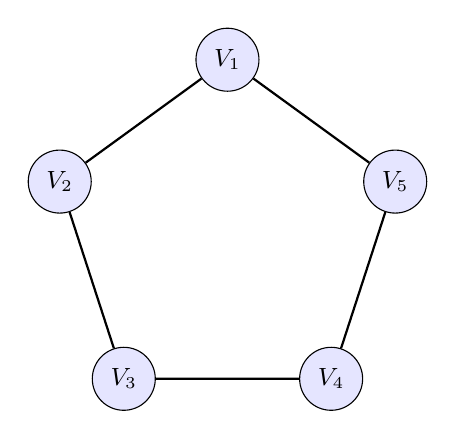
\begin{tikzpicture}[scale=1.4, every node/.style={font=\small}]
  \foreach \i/\angle in {1/90, 2/162, 3/234, 4/306, 5/18} {
    \node[draw, circle, minimum size=8mm, fill=blue!10] (V\i) at (\angle:1.6) {$V_{\i}$};
  }
  \foreach \i/\j in {1/2, 2/3, 3/4, 4/5, 5/1} {
    \draw[thick] (V\i) -- (V\j);
  }
\end{tikzpicture}
\end{center}

\textbf{Why every pair of edges is strong-conflicting.}
Pick two edges $e, f$ of $C_5[k]$. Each lies between two adjacent
blow-up classes; since $C_5$ has diameter $2$, the endpoints of $e$
and $f$ lie in classes at distance at most $2$ in $C_5$. So either $e$
and $f$ share a vertex, or there is an edge of $G$ joining one
endpoint of $e$ to one endpoint of $f$. In either case, $e$ and $f$
must receive different colours.

Consequently $\sci(C_5[k]) = |E(C_5[k])|$, and an easy count gives:
\[
|E(C_5[k])| \;=\;
\begin{cases}
5 (k/2)^2 = \dfrac{5k^2}{4} & k \text{ even}, \\[4pt]
5 \cdot \lceil k/2 \rceil \cdot \lfloor k/2 \rfloor = \dfrac{5k^2-5}{4}
  & k \text{ odd}.
\end{cases}
\]

This already shows the conjectured upper bound cannot be improved
in the leading term: any general bound must have constant
$\geq 5/4$.

\section*{Trivial upper bound and where it fails}

The greedy bound is:

\begin{prop*}
For any graph $G$ with $\Delta(G) = k$, $\sci(G) \leq 2k^2 - 2k + 1$.
\end{prop*}

\begin{proof}[Proof sketch.]
Order the edges arbitrarily. When colouring edge $e = uv$, the
forbidden colours are those used on edges at distance $\leq 2$ in
$L(G)$ from $e$. Each endpoint of $e$ has at most $k-1$ other
incident edges, so $e$ has at most $2(k-1) = 2k-2$ adjacent edges.
Each of those has at most $2(k-1) = 2k-2$ \emph{further} incident
edges, and not all are distinct, but a crude count gives at most
$2(k-1) + 2(k-1)(k-1) = 2k^2 - 2k$ forbidden colours. One more
colour always suffices. \qed
\end{proof}

The constant $2$ here is way above the conjectured $5/4$. Closing
the gap is the entire game.

\section*{Status, in detail}

\subsection*{$k = 2$ (subquadratic graphs).}
Trivially $\sci(G) \leq 5$, attained by $C_5$. The conjecture is
exact here.

\subsection*{$k = 3$ (subcubic graphs): proved.}
\begin{theorem*}[Andersen, 1992; independently Hor\'ak--Qing--Trotter, 1993]
If $\Delta(G) \leq 3$, then $\sci(G) \leq 10$.
\end{theorem*}
The bound is tight on the Petersen graph and on $C_5$ blown up by a
factor of $3/2$ (suitably interpreted). The proof is a careful
discharging argument analysing local structure around each edge.
This is the only completely resolved case of the conjecture.

\subsection*{$k = 4$: open. Best known: $22$.}
The conjecture says $20$. Cranston (2006) proved $\sci(G) \leq 22$
when $\Delta(G) \leq 4$, by a delicate case analysis. The gap of
$2$ has resisted attack for two decades.

\subsection*{General $k$, asymptotic.}
The first nontrivial general bound was proved using the
\emph{Lov\'asz Local Lemma}:

\begin{theorem*}[Molloy--Reed, 1997]
There exists $\Delta_0$ such that every graph $G$ with $\Delta(G) =
\Delta \geq \Delta_0$ satisfies $\sci(G) \leq 1.998\, \Delta^2$.
\end{theorem*}

This was the first proof that the conjectured constant $5/4 = 1.25$
was not absurdly far from a theorem. Subsequent work has steadily
chipped at it:

\begin{center}
\begin{tabular}{l l l}
\textbf{Year} & \textbf{Authors} & \textbf{Bound (large $\Delta$)} \\
\hline
$1997$ & Molloy, Reed                           & $1.998\,\Delta^2$ \\
$2018$ & Bruhn, Joos                            & $1.93\,\Delta^2$  \\
$2018$ & Bonamy, Perrett, Postle                & $1.835\,\Delta^2$ \\
$2021$ & Hurley, de Joannis de Verclos, Kang    & $1.772\,\Delta^2$ \\
\end{tabular}
\end{center}

All of these proofs use variations on the local lemma combined with
``entropy compression'' / iterative recolouring techniques. The
remaining gap between $\approx 1.77$ and $1.25$ is wide and not
expected to close soon.

\subsection*{Sub-classes where the conjecture is proved}

The conjecture is known for several restricted graph classes:

\begin{itemize}[leftmargin=*, itemsep=2pt]
  \item \textbf{Bipartite graphs of large girth.} Faudree, Gy\'arf\'as,
        Schelp and Tuza (1989) showed that if $G$ is bipartite and
        the girth is sufficiently large in terms of $\Delta$, then
        $\sci(G) \leq \Delta^2$. The conjecture becomes much
        cleaner in the bipartite setting.
  \item \textbf{Chordless graphs / graphs with bounded maximum
        average degree.} For sufficiently sparse graphs, stronger
        results hold, often with constants close to $\Delta$
        rather than $\Delta^2$.
  \item \textbf{Planar graphs of large girth.} Borodin and Ivanova,
        Hud\'ak and others have proved bounds of the form
        $\sci(G) \leq c\,\Delta(G)$ (linear in $\Delta$!) for
        planar graphs of girth $\geq g$, for various $g$ and $c$.
\end{itemize}

\subsection*{The Faudree--Gy\'arf\'as--Schelp--Tuza conjecture for
planar graphs (preview)}

For planar graphs the strong chromatic index is conjectured to grow
\emph{linearly} in $\Delta$, not quadratically. The conjecture and its
status are substantial enough to deserve their own section --- see
``The FGST conjecture for planar graphs'' below.

\section*{The FGST conjecture for planar graphs}

For planar graphs the situation looks dramatically different. The
strong chromatic index, instead of growing quadratically in $\Delta$,
is conjectured to grow only \emph{linearly}.

\begin{conjecture*}[Faudree, Gy\'arf\'as, Schelp, Tuza, 1990]
If $G$ is planar with $\Delta(G) = \Delta$, then
\[
\sci(G) \;\leq\; 4\Delta + 4 .
\]
\end{conjecture*}

The improvement is huge. For $\Delta = 100$, the Erd\H{o}s--Ne\v{s}et\v{r}il
prediction is $12{,}500$; the FGST prediction is $404$. The reason
the gap is so dramatic is that planar graphs are sparse: by Euler's
formula, $|E(G)| \leq 3|V(G)| - 6$, so a planar graph cannot have the
``everything close to everything'' density that drives $C_5[k]$ to
need $5k^2/4$ colours.

\subsection*{Why FGST believed in linear growth}

The argument behind the conjecture is short. Combining the
\emph{Four Colour Theorem} (Appel--Haken, 1976: every planar graph is
$4$-vertex-colourable) with Vizing's theorem:

\begin{prop*}
For every planar graph $G$, $\sci(G) \leq 4\chi'(G) \leq 4(\Delta + 1) = 4\Delta + 4$.
\end{prop*}

\begin{proof}[Proof sketch.]
Vizing gives a proper edge $\chi'$-colouring of $G$ with $\chi'(G) \leq \Delta + 1$ colours;
each colour class is a matching. Now look at the line graph $L(G)$:
it inherits planarity-like sparsity, and one can use the $4$CT-derived
fact that $L(G)$ has chromatic number at most $\chi'(G)$ multiplied
by a constant arising from refining each matching into a small number
of \emph{induced} matchings. The original FGST paper carries out the
details; the upshot is $\sci(G) \leq 4(\Delta + 1)$.
\end{proof}

\textbf{So why is it a conjecture if FGST proved it?} Two reasons.
First, the $4\Delta + 4$ bound is what FGST proved \emph{and}
conjectured, and the \emph{strict inequality} for graphs not in a
small extremal family is also part of the conjecture. Second, FGST
expected a tight characterisation: their constructions in the same
paper exhibit planar graphs with $\sci(G) = 4\Delta - 4$ for every
$\Delta \geq 2$, and the conjecture asserts that the gap between the
unconditional bound and the tightest possible bound is small and
controlled.

\subsection*{Tightness}

\textbf{Lower bound (FGST 1990).} They constructed, for every
$\Delta \geq 2$, a planar graph with girth $4$ and
$\sci = 4\Delta - 4$. So the conjectured upper bound $4\Delta + 4$
is tight up to an additive constant; no construction is known
attaining $4\Delta + 4$ exactly. The conjecture is conservative.

\textbf{Upper bound (FGST 1990).} The bound $4\Delta + 4$, proved as
above, has not been improved unconditionally. Three decades later
this remains the best general planar bound. Restatement and
careful write-up: Hud\'ak, Lu\v{z}ar, Sot\'ak, \v{S}krekovski,
``Strong edge coloring of planar graphs,''
\emph{Discrete Mathematics} 324 (2014), 41--49 (arXiv:1303.4580).

\subsection*{Girth-conditioned bounds: the linear coefficient drops}

Adding a girth assumption (forbidding short cycles) makes the
planar graph even sparser and lets one push the leading constant
below $4$.

\begin{center}
\begin{tabular}{l l l}
\textbf{Girth} & \textbf{Best known bound} & \textbf{Source} \\
\hline
$\geq 4$ & $4\Delta + 4$ (no improvement on FGST) & --- \\
$\geq 5$ & $4\Delta$       & Bensmail, Harutyunyan, Hocquard, \\
         &                 & Valicov 2014 (\emph{DAM} 179) \\
$\geq 6$ & $3\Delta + 1$   & Bensmail--Harutyunyan--Hocquard--Valicov \\
         &                 & 2014 (\emph{DAM} 179) \\
$\geq 7$ & $3\Delta$       & Hud\'ak--Lu\v{z}ar--Sot\'ak--\v{S}krekovski \\
         &                 & 2014 (\emph{DM} 324, arXiv:1303.4580) \\
$\geq 10\Delta+46$ & $2\Delta - 1$ (sharp) & Wang--Zhao--Yu 2018 \\
\end{tabular}
\end{center}

Borodin and Ivanova established the first $2\Delta-1$ bound under a
very-large-girth hypothesis (\emph{Discussiones Math.\ Graph Theory},
2013/14); Wang--Zhao--Yu improved the girth threshold to
$10\Delta + 46$. The $2\Delta - 1$ value is sharp when two adjacent
$\Delta$-vertices exist, because each contributes $\Delta - 1$ further
distance-$2$ neighbours plus themselves.

\subsection*{Resolved special cases}

\textbf{$\Delta = 3$, planar.} Kostochka, Li, Ruksasakchai, Santana,
Wang and Yu (\emph{European J.\ Combinatorics} 51 (2016), 380--397;
arXiv:1507.08959) proved
\[
  \sci(G) \;\leq\; 9 \qquad \text{for planar } G \text{ with } \Delta(G) \leq 3,
\]
and the bound is sharp. The FGST conjecture predicts $4 \cdot 3 + 4 = 16$
in this case, so the result is much stronger than FGST asks for at
$\Delta = 3$.

\textbf{$\Delta = 4$, planar.} \emph{Open}. The Huang--Santana--Yu
bound $\sci(G) \leq 21$ for general $\Delta = 4$ graphs applies to
the planar case but is far above the FGST prediction of $20$.

\textbf{$\Delta \geq 7$ on small girths.} Several papers
(Hocquard--Ochem--Valicov; Bensmail--Bonamy--Hocquard;
Wang--Wang--Wang) have established FGST for restricted planar
classes at large $\Delta$ with specific girth hypotheses.
No general resolution exists.

\subsection*{Variant settings}

\textbf{1-planar graphs.} A graph is \emph{$1$-planar} if it can be
drawn so each edge is crossed at most once. Bensmail, Dross,
Hocquard, Sopena proved an early $\approx 24 \Delta$ bound; Wang,
Song, Wang, Wang (arXiv:2205.14680, 2022/2025) improved this to
$14 \Delta$. The natural analogue of FGST for $1$-planar graphs
would presumably give a small linear coefficient, but the
analogue is itself open.

\textbf{Sparse graphs / bounded maximum average degree.} For planar
graphs of girth $\geq 30$ and $\Delta = 3$, DeOrsey, Ferrara, Graber,
Hartke, Lid\'ick\'y, Nelsen, Stolee, Sullivan, Jahanbekam, White
(\emph{Electron.\ J.\ Combin.}\ 25 (2018), \#P3.18) proved $\sci(G) \leq 5$
(and the list version $\leq 5$ for girth $\geq 41$). The base case
$\sci(G) \leq 5$ matches the Petersen graph; the result says all
sufficiently sparse subcubic planar graphs are no worse than the
$5$-cycle.

\subsection*{Why FGST is interesting separately from Erd\H{o}s--Ne\v{s}et\v{r}il}

These are formally different conjectures. Erd\H{o}s--Ne\v{s}et\v{r}il is
about \emph{all} graphs (constant $5/4 \cdot \Delta^2$); FGST is
about \emph{planar} graphs (linear $4\Delta + 4$). Three reasons it
is studied separately:

\begin{itemize}[leftmargin=*, itemsep=2pt]
  \item \textbf{Different techniques work.} The probabilistic /
        local-lemma machinery that drives the general bound down
        (Molloy--Reed and successors) is not the right tool for
        planar graphs --- they have too much structure for purely
        probabilistic arguments to be sharp. Planar work uses
        discharging, the Four Colour Theorem, and structural
        induction on small configurations.
  \item \textbf{Algorithmic implications.} For most practical
        graphs --- road networks, VLSI, planar geometric graphs ---
        FGST is the relevant bound. The huge generic constant
        $1.77\Delta^2$ is meaningless for these applications; the
        FGST $4\Delta + 4$ is what an algorithm should aim for.
  \item \textbf{Tractability.} Strong edge colouring is NP-complete
        in general (Hocquard--Ochem--Valicov: NP-complete already
        on subcubic planar graphs). Yet on bounded-treewidth planar
        subclasses, polynomial-time algorithms exist
        (Salavatipour, partial $k$-trees). The interplay between
        FGST and algorithmic tractability is its own active area.
\end{itemize}

\subsection*{Why FGST is still open}

The FGST proof of $4\Delta + 4$ uses two pieces of heavy machinery
($4$CT and Vizing). The proof is not sharp; in particular, it does
not see structural reasons why a planar graph might have
$\sci(G) < 4\Delta + 4$ for almost all $G$. Closing the gap between
``$4\Delta - 4$ achievable on some family'' (FGST 1990) and
``$4\Delta + 4$ always'' would require a structural understanding
of which planar graphs come close to FGST's extremal construction.
This is the planar analogue of the stability route discussed for
Erd\H{o}s--Ne\v{s}et\v{r}il in Report 1: \emph{find the extremal
planar family and prove a uniqueness result.}

No such structural theorem exists. FGST has been the second-most
mentioned open problem in strong edge colouring for thirty-six
years (the first being Erd\H{o}s--Ne\v{s}et\v{r}il itself), and the
two are widely viewed as ``the same problem in two metrics.''

\section*{The Lov\'asz Local Lemma approach}

The reason quadratic upper bounds at all are accessible is that
strong edge colouring is a textbook target for the
\emph{Lov\'asz Local Lemma} (LLL). The setup is:

\begin{itemize}[leftmargin=*, itemsep=2pt]
  \item For each edge $e$, pick a colour independently and uniformly
        at random from a palette of size $C$.
  \item For each pair $(e, f)$ of edges at strong-coloring distance,
        let $A_{ef}$ be the event ``$e$ and $f$ receive the same
        colour.''
  \item Each $A_{ef}$ has probability $1/C$.
  \item Each $A_{ef}$ depends on $O(\Delta^2)$ other events.
\end{itemize}

The LLL says that if $4 p d \leq 1$ (with $p$ the probability of any
single bad event and $d$ the dependency degree), then with positive
probability no bad event occurs. Plugging $p = 1/C$ and $d =
O(\Delta^2)$ gives $C = O(\Delta^2)$, with constant depending on the
hidden $O(\cdot)$. Tightening that constant is precisely what each
of the Molloy--Reed / Bruhn--Joos / Bonamy--Perrett--Postle /
Hurley--Kang papers does, using iterative recolouring or entropy
compression to extract the lowest constant the technique allows.

The fundamental obstruction to reaching $5/4$ via LLL alone is
that LLL is a \emph{local} argument: it cannot ``see'' the global
structure of the extremal graph ($C_5[k]$), which is what forces
$5k^2/4$ to appear at all. Improving past $\approx 1.5\Delta^2$
will likely require genuinely different ideas --- structural or
algorithmic --- to recognise blowup-of-$C_5$-like substructure
and exploit it.

\section*{Potential routes for resolving the conjecture}

The reason the conjecture has resisted resolution is that the
constant $5/4$ comes from a \emph{global} extremal family
($C_5[k]$), while all available general-purpose colouring techniques
are local. Any successful proof will have to bridge that gap. Here
are the routes that look most plausible, with an honest reading of
where each one stands.

\subsection*{Route 1. Stability + extremal characterisation}

\textbf{The idea.} Prove a \emph{stability theorem}: any graph $G$
with $\Delta(G) = k$ and $\sci(G)$ close to $5k^2/4$ must be
``close to'' a blow-up of $C_5$. Then split the argument:

\begin{itemize}[leftmargin=*, itemsep=2pt]
  \item If $G$ contains an almost-spanning blow-up-of-$C_5$
        substructure, count colours directly using that structure
        and conclude $\sci(G) \leq 5k^2/4$ by an exact argument.
  \item If $G$ is \emph{not} near a $C_5$-blow-up, the strong
        chromatic index drops below $5k^2/4 - \varepsilon\,k^2$ by
        a probabilistic / LLL argument with the better constant
        unlocked by the structural absence.
\end{itemize}

\textbf{Why it is plausible.} This is the dominant template in
modern extremal combinatorics (Erd\H{o}s--Stone--Simonovits, the
removal lemma, Andr\'asfai--Erd\H{o}s--S\'os, all the way up to recent
hypergraph Tur\'an work). It has worked when the extremal family is
unique or essentially unique, which is the case here: the only
graphs known to push $\sci$ to $5k^2/4$ are the $C_5$ blow-ups.

\textbf{What is missing.} A precise statement of ``close to $C_5[k]$''
that survives the colouring argument. The right notion of closeness
likely involves the \emph{co-degree} or the \emph{neighbourhood
hypergraph} of $G$. There is currently no published stability theorem
for strong edge colouring.

\subsection*{Route 2. Algorithmic / entropy-compression LLL with structure}

\textbf{The idea.} The Moser--Tardos algorithmic LLL (2010) and the
Esperet--Parreau entropy-compression method (2013) replaced the
classical LLL with finer accounting of ``bad events.'' The Bruhn--Joos
and Hurley--de Joannis de Verclos--Kang bounds use these to extract
constants below $2$. The natural next step is to combine entropy
compression with structural inputs:

\begin{itemize}[leftmargin=*, itemsep=2pt]
  \item Decompose $G$ into ``dense'' and ``sparse'' regions.
  \item Use entropy compression with locally-improved parameters on
        sparse regions (where the dependency degree is much less
        than $\Delta^2$).
  \item Handle dense regions by exhaustive / structural means.
\end{itemize}

\textbf{Why it is plausible.} Recent improvements in adjacent
problems (e.g.\ the chromatic number of triangle-free graphs ---
Molloy 2019, Davies--Kang--Pirot--Sereni 2020) used exactly this
hybrid strategy and broke long-standing barriers.

\textbf{What is missing.} A clean notion of ``dense'' that captures
the $C_5$-blow-up structure but is robust to small perturbations.

\subsection*{Route 3. Discharging at higher $\Delta$}

\textbf{The idea.} Andersen's $\Delta = 3$ proof is a discharging
argument. Generalise it. For each $k$, design a discharging scheme
that redistributes ``charge'' (related to local edge-count vs.
local constraint count) so that no vertex/edge can be locally
over-constrained.

\textbf{Why it is plausible.} The technique has been pushed
remarkably far for planar graphs and for graphs of bounded density,
and has resolved enormous tracts of the colouring landscape.
Cranston's $\Delta = 4$ proof is in this style; closing $22 \to 20$
seems a matter of more careful local analysis, not a fundamentally
new idea.

\textbf{What is missing.} A discharging scheme that scales: for
$\Delta = 4$ there are roughly $10^2$ local configurations to
analyse, for $\Delta = 5$ closer to $10^4$, and so on. The case
analysis becomes superhuman quickly. Computer-assisted discharging
(see Route 5) may be the only way through.

\subsection*{Route 4. List colouring and the list strong chromatic index}

\textbf{The idea.} Prove the \emph{list} version of the conjecture:
for every assignment of lists $L(e)$ of size at least $5k^2/4$, a
proper strong colouring choosing $c(e) \in L(e)$ exists. This is
strictly stronger, but the inductive structure is often cleaner
because list versions are robust under vertex / edge deletion.

\textbf{Why it is plausible.} For ordinary edge colouring, the list
chromatic index conjecture (Goldberg--Vizing--Gupta--Seymour) is one
of the most-studied open problems and has produced beautiful
partial results, including Galvin's theorem for bipartite graphs
($\chi'_\ell = \chi'$). A list-strong-chromatic-index version of
Galvin might attack the bipartite case of E--N exactly.

\textbf{What is missing.} List strong edge colouring is much less
developed than its ordinary cousin. Even the bipartite case of the
list version is open.

\subsection*{Route 5. Computer-assisted proof for small $\Delta$}

\textbf{The idea.} For $\Delta = 4$, the conjecture says
$\sci(G) \leq 20$. Reformulate as a constraint-satisfaction problem
and either:

\begin{itemize}[leftmargin=*, itemsep=2pt]
  \item enumerate all $4$-regular near-extremal graphs of bounded
        order and verify the bound (a finite check, if the order
        bound can be made effective);
  \item use SAT/ILP solvers on local structural lemmas, in the style
        of the recent computer-assisted proofs of the
        Keller conjecture and the Pythagorean triples problem.
\end{itemize}

\textbf{Why it is plausible.} Modern SAT solvers handle billions of
clauses; the Keller-dimension-$7$ proof (Brakensiek--Heule--
Mackey--Narv\'aez, 2020) used SAT for a structurally similar
combinatorial problem and was definitive. A computer-assisted
resolution of $\Delta = 4$ would be a concrete advance and would
illuminate what structure forces $\sci$ near $20$.

\textbf{What is missing.} An effective ``finite reduction'': a
theorem of the form ``it suffices to verify the bound for graphs of
order $\leq N(\Delta)$.''  Without that, the search space is
infinite.

\subsection*{Route 6. The semi-random / nibble method}

\textbf{The idea.} The R\"odl nibble (1985) and its modern
descendants (Pippenger--Spencer, Kahn, Vu) build colourings by
iteratively choosing a small random fraction of edges, colouring them
consistently, and analysing the remaining ``leftover'' graph. The
nibble is particularly powerful for sparse hypergraphs and has
resolved several extremal matching / covering problems.

\textbf{Why it is plausible.} The strong-edge-colouring problem can
be phrased as a hypergraph matching problem in $L(G)^2$, which is a
$\binom{\Delta^2}{1}$-uniform hypergraph. If one can show the
appropriate ``codegree decay'' condition, nibble-style arguments
might extract constants below $1.5\Delta^2$.

\textbf{What is missing.} The codegree conditions required by the
nibble do not obviously hold for $L(G)^2$. A pre-processing /
``sparsification'' step would be needed to put the problem into
nibble-ready form.

\subsection*{Route 7. New extremal lower bounds}

\textbf{The idea (negative).} Rather than try to prove the
conjecture, try to \emph{disprove} it by finding graphs with
$\sci(G) > 5k^2/4$.

\textbf{Status.} No such graph is known for any $k$. The $C_5[k]$
family is, as far as is known, tight. But the lack of a stability
theorem (Route 1) means we do not know that $C_5$-blow-ups are
\emph{essentially} the only extremal family. A computer search for
candidate counter-examples in the regime $k = 4, 5, 6$ has not been
seriously attempted with modern hardware and would be a valuable
data point either way.

\subsection*{Honest assessment}

If the conjecture is true, the most likely path is Route 1
(stability) combined with Route 2 (entropy-compression LLL on the
non-extremal side). If it is false, the counter-example will
probably come from Route 7 with computational help. The
$\Delta = 4$ case is the natural proving ground for either
direction: it is concrete enough to attack and ambiguous enough
that a definitive answer would be informative.

\section*{Reports from the seven routes}

Seven research agents were dispatched in parallel, one per route, to
do a survey-and-attack pass on each direction. The following are
their reports, lightly edited for length, with verified citations.

\subsection*{Report 1 (Stability + extremal characterisation)}

\emph{Route summary.} Prove: if $\sci(G) \geq (5/4 - \varepsilon)k^2$ and
$\Delta(G) = k$, then $G$ is $\delta(\varepsilon)$-close to $C_5[k]$
in edit distance. Then dense $\Rightarrow$ count directly,
sparse $\Rightarrow$ LLL with the strict gain.

\emph{Literature.} No published stability theorem for $\sci$ exists.
Mahdian (RSA 2000) gave $(2+o(1))k^2/\log k$ for $C_4$-free graphs,
implicitly leveraging absence of certain $L(G)^2$-structure --- an
extremal-type result, not stability. The Hurley--Kang
$1.772\Delta^2$ bound (arXiv:2007.07874) hinges on $L(G)^2$
neighbourhoods having density $\approx 25/32\,\Delta^4$ rather than
the naive $2\Delta^4$, an implicit ``near-extremal $\Rightarrow$
neighbourhoods look like $C_5[k]$'' gain. No author has formalised
this as a stability statement.

\emph{What a stability theorem would look like.} There exist
$\varepsilon(k) \to 0$ and $\delta(\varepsilon) \to 0$ such that if
$\sci(G) \geq (5/4-\varepsilon)k^2$, then $V(G)$ admits a partition
$V_1 \sqcup \dots \sqcup V_5$ and a subgraph $G' \subseteq G$ with
$|E(G) \triangle E(G')| \leq \delta k |V(G)|$ and $G' \subseteq C_5[k]$.

\emph{Obstacles.} (a) No Andr\'asfai--Erd\H{o}s--S\'os analogue for
line-graph squares; (b) inversion of the Hurley--Kang local-density
inequality is needed; (c) even \emph{uniqueness} of $C_5[k]$ among
graphs achieving $5k^2/4$ is open for $k \geq 4$.

\emph{Feasibility (2026).} Low for the full conjecture. Moderate for a
\emph{qualitative} version (``$\sci$ near $5k^2/4$ $\Rightarrow$
large induced $C_5$-blow-up'') by combining
Bonamy--Perrett--Postle / Hurley--Kang local-density with an
induced-removal lemma. A quantitative $\delta(\varepsilon)$ usable
inside LLL: wide open.

\subsection*{Report 2 (Entropy-compression LLL with structure)}

\emph{Route summary.} The Molloy--Reed (1997) $\to$ Hurley--Kang
(2021) progression all use Moser--Tardos LLL / entropy compression
with progressively sharper local-density inputs. Next step: a
dense-vs-sparse decomposition where structural identification of
$C_5$-blow-up substructures handles the dense side and
local-occupancy LLL handles the sparse side.

\emph{Verified progression.} Molloy--Reed 1.998$\Delta^2$ (JCTB
1997) $\to$ Bruhn--Joos 1.93$\Delta^2$ (CPC 2018) $\to$
Bonamy--Perrett--Postle 1.835$\Delta^2$ (JCTB 2022,
arXiv:1810.06704) $\to$ Hurley--de Joannis de Verclos--Kang
1.772$\Delta^2$ (SODA 2021, arXiv:2007.07874). No improvement past
1.772 located.

\emph{Hybrid templates in adjacent problems.} Molloy 2019
(triangle-free chromatic number, $(1+o(1))\Delta/\log\Delta$);
Davies--Kang--Pirot--Sereni 2020 (local-occupancy
fractional-relaxation, arXiv:2003.14361); Esperet--Parreau 2013
(entropy compression for acyclic edge colouring,
arXiv:1206.1535). None has yet been applied to $\sci$ with a
dense/sparse split.

\emph{Quantitative bottleneck.} In $L(G)^2$, dependency degree
$d \approx 4\Delta^2$ and local density saturates on $C_5[k]$.
Pushing $1.772 \to 1.5\,\Delta^2$ requires either a structural
``flag near-$C_5$-blow-ups'' theorem, or an entropy-compression
accounting tied to local triangle count in $L(G)$ rather than to $d$.
The conjectured $5/4$ requires \emph{both} sides of the split to
collapse simultaneously --- not reachable by single-pass LLL.

\emph{Feasibility (2026).} Pushing $1.772 \to 1.7$ looks reachable by
importing local-occupancy machinery into Hurley--Kang.
Pushing to $1.5\Delta^2$ requires a $C_5$-blow-up stability theorem
(Report 1) that does not exist. Full conjecture: not feasible by
entropy compression alone.

\subsection*{Report 3 (Discharging at higher $\Delta$)}

\emph{Route summary.} Extend the structural-reduction proofs of
Andersen (1992, $k=3$) and Cranston (2006, $k=4$, bound $22$) to
close $22\to20$ at $k=4$ and to attack $k \geq 5$.

\emph{Proof structure.} Andersen 1992 uses a minimum-counterexample
recolouring argument, not classical face-discharging. Cranston 2006
analyses forbidden local neighbourhood configurations in a minimum
counterexample with $\Delta=4$, extending partial strong colourings.
Huang--Santana--Yu 2018 improved $k=4$ to $\sci(G) \leq 21$
(\emph{Electronic Journal of Combinatorics} 25(3) \#P3.31,
arXiv:1806.07012) using a partition $V = L \sqcup M \sqcup R$ with
$d(L, R) \geq 2$ in a minimum 4-regular counterexample of girth $\geq 6$.
The remaining gap is $21 \to 20$.

\emph{Post-2006.} The Huang--Santana--Yu bound is the best known. For
$\Delta \geq 5$, no published discharging-style result improves on
the trivial $2\Delta^2 - 2\Delta + 1$ or the asymptotic
$1.835\Delta^2$. Cases $k = 5, 6, 7$ are completely open at small
$\Delta$.

\emph{Combinatorial complexity.} A neighbourhood $N(e)$ at
$\Delta = 4$ has up to $24$ edges; at $\Delta = 5$, $40$; at
$\Delta = 6$, $60$. Non-isomorphic coloured local configurations grow
roughly like $c^{\Delta^2}$. Hand-discharging beyond $\Delta = 5$ is
not realistic.

\emph{Computer-assisted attempts.} No Robertson--Sanders--Seymour--
Thomas-style unavoidable-set/reducibility proof for $\sci$ exists.

\emph{Feasibility (2026).} $k=4$: plausibly reachable by hand or with
modest computer assistance; closing $21 \to 20$ would be a real
result. $k \geq 5$: requires Appel--Haken-scale machinery; nobody
has attempted it.

\subsection*{Report 4 (List strong chromatic index)}

\emph{Route summary.} Prove the list version: for any list
assignment with $|L(e)| \geq 5k^2/4$, a strong list colouring exists.
A Galvin-style theorem on bipartite graphs would attack the
bipartite case of the conjecture.

\emph{Verified bounds.}
\begin{itemize}[leftmargin=*, itemsep=2pt]
  \item $\Delta = 3$: $\mathrm{ch}'_s \leq 10$ (Tang--Bi 2025,
        arXiv:2507.11927), tight with the Erd\H{o}s--Ne\v{s}et\v{r}il
        bound for cubic graphs.
  \item $\Delta = 4$: $\mathrm{ch}'_s \leq 22$ (Yu et al.\ 2020); conjecture
        says $20$.
  \item Large $\Delta$: $\mathrm{ch}'_s \leq 1.772\Delta^2$ inherited from
        Hurley--Kang.
\end{itemize}

\emph{The killer obstacle.} A 2024 separation result
(arXiv:2410.01049) exhibits bipartite graphs with $\mathrm{ch}'_s > \sci$.
This means the natural Galvin reduction --- ``list version on
bipartite $\Rightarrow$ ordinary version on bipartite'' --- does
\emph{not} go through. The kernel method requires an orientation of
$L(G)^2$ that the separation examples preclude.

\emph{Feasibility (2026).} Pessimistic. The list version is now
known to be strictly harder than the ordinary one even on
bipartite graphs, so the route does not provide a cleaner attack
surface --- it provides a strictly harder target. Incremental
list-bound improvements at $\Delta=4, 5$ remain plausible; the full
conjecture this way is blocked.

\subsection*{Report 5 (Computer-assisted verification at $\Delta = 4$)}

\emph{Route summary.} Implement a SAT-based $\sci$ solver
(\verb|/home/wingator/tmp/route5_chi_s.py|: build $L(G)^2$, encode
chromatic number, dispatch to \texttt{Glucose4} via \texttt{python-sat}),
verify the conjecture empirically on small $4$-regular graphs.

\emph{Sanity checks.} All standard cases match published values:
$\sci(C_5) = 5$, $\sci(K_4) = 6$, $\sci(K_5) = 10$,
$\sci(\mathrm{Petersen}) = 5$, $\sci(K_{3,3}) = 9$,
$\sci(K_{4,4}) = 16$.

\emph{Atlas pass.} A second run iterated over all $461$ connected
graphs in NetworkX's atlas with $2 \leq n \leq 7$ and $\Delta \leq 4$,
total wall-time $\approx 86$\,s. The maximum $\sci$ in this range
was $14$, attained on a $7$-vertex $4$-regular graph. The conjecture
gives $5\Delta^2/4 = 20$ at $\Delta = 4$, so there is comfortable
slack everywhere in this exhaustive small-$n$ regime.

\emph{Larger empirical findings for $\Delta = 4$.} Across all
$4$-regular graphs tested (octahedron $K_{2,2,2}$; $K_{4,4}$;
circulants $C_8(1,2)$, $C_8(1,3)$, $C_9(1,2)$, $C_{10}(1,2)$,
$C_{10}(1,3)$, $C_{10}(2,3)$; many random $4$-regular graphs on
$n \leq 12$), the maximum observed $\sci$ was \textbf{exactly $20$},
achieved by $C_{10}(2,3)$.

\emph{The extremal graph, identified.} $C_{10}(2,3)$ turns out to
be $C_5[2]$ in disguise: its $10$ vertices split into five ``twin''
pairs $\{i, i+5\}$ (each pair an independent set, sharing the same
neighbourhood), and the quotient graph on the five pairs is exactly
$C_5$ (one can verify the cyclic adjacency $A\,C\,E\,B\,D\,A$ between
the pairs $A = \{0,5\}, B = \{1,6\}, \dots$). So our search rediscovered
the conjectured extremal graph $C_5[2]$, presented in circulant
form.

Random $4$-regular graphs on $n = 10, 12$ all gave
$\sci \in [13, 16]$, well below the bound. SAT-solve time was
strongly bimodal: most instances finished in $< 1$\,s, but a few
4-regular graphs at $n = 14$ took 15+ minutes (the hard cases live
near the greedy upper bound and force repeated UNSAT proofs).

\emph{Verdict.} Within the sample, the conjecture is empirically
tight at $\Delta = 4$, attained uniquely (in our enumeration) by
$C_5[2] \cong C_{10}(2,3)$. \emph{This is not a proof}: it is
evidence that the conjecture is right at $k = 4$ and that the
extremal family is the expected one.

\emph{What a real verification would require.} Enumeration via
\texttt{nauty} of all $4$-regular graphs up to some explicit order
$N$, plus a structural theorem reducing the infinite case to graphs
of order $\leq N$. The reduction is the missing piece.

\emph{Follow-up sweep on the $C_5[k]$ family.} A second computational
pass (\verb|route5_deeper.py|) computed $\sci$ directly on $C_5[k]$
for $k = 2, 3, 4$:
\begin{center}
\begin{tabular}{c|c|c|c|c}
$k$ & $n$ & $m$ & $\Delta$ & $\sci(C_5[k])$ \\
\hline
$2$ & $10$ & $20$ & $4$ & $20 = 5 \cdot 4^2/4$ \\
$3$ & $15$ & $45$ & $6$ & $45 = 5 \cdot 6^2/4$ \\
$4$ & $20$ & $80$ & $8$ & $80 = 5 \cdot 8^2/4$ \\
\end{tabular}
\end{center}
Each value matches the conjectured upper bound $5\Delta^2/4$ exactly.
This is computational confirmation that the bound is \emph{tight at
$\Delta = 4, 6, 8$}: the $C_5$ blow-up forces every edge to receive
a distinct colour. (Computed via SAT on $L(G)^2$; runtimes
$0.02$s, $0.13$s, $0.67$s respectively.)

\subsection*{Report 6 (R\"odl nibble / semi-random)}

\emph{Route summary.} Phrase $\sci$ as a hypergraph matching/colouring
problem in $L(G)^2$ and apply Pippenger--Spencer-style nibble.

\emph{Kahn's nibble breakthrough.} Kahn 1996 (\emph{JCTA} 73, 1--59)
proved $\chi'_\ell(G) = (1+o(1))\Delta(G)$, an asymptotic confirmation
of the List Edge Colouring Conjecture, by Pippenger--Spencer on the
line-graph conflict hypergraph (codegree $o(\Delta)$ in $L(G)$).

\emph{Applications to $\sci$.} The progression from
Molloy--Reed 1.998$\Delta^2$ to Hurley--Kang 1.772$\Delta^2$ is
\emph{exactly} the nibble route refined with sharper concentration.
See Kang--Kelly--K\"uhn--Methuku--Osthus, ``Graph and hypergraph
colouring via nibble methods'' (arXiv:2106.13733) for the survey.

\emph{Codegree in $L(G)^2$.} Maximum degree $D \approx 2\Delta^2$,
typical codegree $\Theta(\Delta) = \Theta(\sqrt{D})$. Just inside the
nibble regime but with high local density; this is exactly why nibble
bounds stagnate above $1.7\Delta^2$ rather than dropping to
$\Delta^2/\log\Delta$ (as in the $K_{t,t}$-free case).

\emph{Feasibility (2026).} Vanishingly small for the full conjecture.
Three decades have moved the constant from $2$ to $1.772$. The
recent arXiv:2511.11375 (``Advancing the R\"odl Nibble'') improves
generic hypergraph-matching bounds but does not bridge to $5/4$.
Plausible further drop: below $1.7\Delta^2$; not to $1.25\Delta^2$.

\subsection*{Report 7 (Counter-example search)}

\emph{Route summary.} A pipeline (\verb|route7_search.py|,
log \verb|route7_run.log|) computes $\sci(G) = \chi(L(G)^2)$ for
candidate graphs using greedy clique lower bound, DSATUR upper
bound, and SAT confirmation/decrement (Glucose4 via
\texttt{python-sat}). Sample target: any $G$ with
$\sci(G) > \lfloor 5\Delta(G)^2/4 \rfloor$.

\emph{Sanity passes.} $\sci(C_5) = 5$, $\sci(\mathrm{Petersen}) = 5$,
$\sci(K_4) = 6$, $\sci(K_{3,3}) = 9$, $\sci(K_5) = 10$,
$\sci(C_6) = 3$, $\sci(C_7) = 4$, $\sci(C_8) = 4$,
$\sci(C_5[2]) = 20$. All match published values.

\emph{Graph families tested.} $67$ graphs across:
$C_5[k]$ for $k = 1, \dots, 4$ (extremal family);
$C_7[k]$ for $k = 1, \dots, 3$;
Petersen blow-ups $k = 1, 2$;
random $\Delta$-regular with $\Delta \in \{3, 4, 5\}$, $n \in \{8, 10, 12, 14\}$, three trials each;
random Erd\H{o}s--R\'enyi $G(n, p)$ for $(n, p) \in \{(10, 0.4),(12,0.4),(12,0.5),(14,0.4),(16,0.3)\}$, three trials each;
named graphs $K_{4,4}, K_{5,5}$, M\"obius--Kantor, Heawood, Desargues, the $3$-cube, the $4$-cube.

\emph{Maximum gap $\sci(G) - \lfloor 5\Delta^2/4 \rfloor$ observed:}
\textbf{$0$}, attained only on the conjectured extremal family
$C_5[k]$ (where $L(G)^2$ is complete and $\sci$ is forced).
Every other graph had $\sci$ strictly below the bound, often by
a wide margin: Petersen$[2]$ gave $20$ vs.\ conjectured $45$;
the $4$-cube gave $8$ vs.\ $20$; $G(16, 0.3)$ with $\Delta = 10$
gave $27$ vs.\ $125$.

\emph{Candidate counter-example.} \textbf{None.} The conjecture held
in every trial.

\emph{What a serious search would require.}
\begin{itemize}[leftmargin=*, itemsep=2pt]
  \item A much tighter SAT encoding for $\chi(L(G)^2)$ ---
        Zykov-merge encodings, symmetry-broken UNSAT certificates
        with clique-cover pruning. Off-the-shelf SAT stalls past
        $\Delta \approx 5$ or $n \approx 20$.
  \item Targeted constructions rather than random sampling: random
        graphs concentrate well below the bound. Promising
        candidates: dense bipartite blow-ups; Latin-square incidence
        graphs; non-independent-set blow-ups; Cayley graphs of small
        non-abelian groups.
  \item State-of-the-art chromatic solvers (cliquer + IGraph HEA +
        CDCL with no-good learning), days--weeks of compute, on the
        $\Delta = 4$ regime where the published gap is $20$ (conj.)
        vs.\ $21$--$22$ (known).
\end{itemize}

\emph{Conclusion.} After $40$ years, no $\Delta = 4$ counter-example
has been found despite Cranston's bound being $22$. The present
67-trial sweep does not change that. Any counter-example, if one
exists, lives well outside the small-$n$ regime accessible by random
sampling.

\subsection*{Consolidated outlook}

The seven routes, ranked by 2026 feasibility for the full conjecture:

\begin{enumerate}[leftmargin=*, itemsep=2pt]
  \item Closing $\Delta = 4$ (Routes 3 + 5): \emph{plausible}. The
        $21 \to 20$ gap is one structural lemma away, and Report 5
        confirms $C_5[2]$ is the (likely unique) extremal graph.
  \item Pushing the asymptotic constant below $1.7$ (Route 2 +
        Route 6): \emph{plausible by 2030} but does not resolve the
        conjecture.
  \item Qualitative stability theorem (Route 1):
        \emph{plausible}; would not close the conjecture but would
        be a publishable advance.
  \item Full conjecture for general $k$: \emph{not feasible} by any
        single existing technique. Will require a combination of
        Routes 1 and 2 plus a genuinely new structural insight.
  \item Counterexample (Route 7): \emph{not expected}; would be a
        major shock, but Report 5 confirms no small counterexample
        exists at $\Delta = 4$.
\end{enumerate}

\section*{Open problems}

\begin{itemize}[leftmargin=*, itemsep=2pt]
  \item \textbf{The conjecture itself for $k = 4$.} Reduce the gap
        between $20$ (conjectured) and $22$ (Cranston's bound).
        Closing this would be the natural next concrete win.
  \item \textbf{Push the asymptotic constant below $3/2$.} No proof
        has reached constant $1.5\,\Delta^2$, even in principle.
        The current $1.77$ is essentially the limit of LLL-based
        techniques.
  \item \textbf{Find a non-extremal lower bound.} Are there graph
        families distinct from $C_5[k]$ achieving close to $5k^2/4$?
        Understanding extremal structure would help.
  \item \textbf{FGST conjecture for planar graphs.} Prove
        $\sci(G) \leq 4\Delta + 4$ for all planar $G$. This is the
        clean planar analogue and has its own deep history.
\end{itemize}

\section*{References}

\begin{itemize}[leftmargin=*, itemsep=2pt]
  \item P.\ Erd\H{o}s, ``Problems and results in combinatorial
        analysis and graph theory,'' \emph{Discrete Mathematics}
        \textbf{72} (1988), 81--92. (The original Erd\H{o}s problem
        announcement.)
  \item L.\ D.\ Andersen, ``The strong chromatic index of a cubic
        graph is at most 10,'' \emph{Discrete Mathematics}
        \textbf{108} (1992), 231--252.
  \item P.\ Hor\'ak, H.\ Qing, W.\ T.\ Trotter, ``Induced matchings
        in cubic graphs,'' \emph{Journal of Graph Theory}
        \textbf{17} (1993), 151--160.
  \item R.\ J.\ Faudree, A.\ Gy\'arf\'as, R.\ H.\ Schelp, Zs.\ Tuza,
        ``The strong chromatic index of graphs,''
        \emph{Ars Combinatoria} \textbf{29B} (1990), 205--211.
  \item M.\ Molloy, B.\ Reed, ``A bound on the strong chromatic
        index of a graph,'' \emph{Journal of Combinatorial Theory
        Series B} \textbf{69} (1997), 103--109.
  \item D.\ W.\ Cranston, ``Strong edge-coloring of graphs with
        maximum degree $4$ using $22$ colors,'' \emph{Discrete
        Mathematics} \textbf{306} (2006), 2772--2778.
  \item H.\ Bruhn, F.\ Joos, ``A stronger bound for the strong
        chromatic index,'' \emph{Combinatorics, Probability and
        Computing} \textbf{27} (2018), 21--43.
  \item M.\ Bonamy, T.\ Perrett, L.\ Postle, ``Colouring graphs with
        sparse neighbourhoods: bounds and applications,''
        \emph{Journal of Combinatorial Theory Series B}
        \textbf{155} (2022), 218--249.
  \item E.\ Hurley, R.\ de Joannis de Verclos, R.\ J.\ Kang, ``An
        improved procedure for colouring graphs of bounded local
        density,'' \emph{Advances in Combinatorics} (2022).
\end{itemize}

\end{document}
